\section*{Цель}

Освоение методов спектрального анализа вариабельности сердечного ритма.

\section*{Порядок выполнения}

\begin{enumerate}
    \item По заданному массиву кардиоинтервалов рассчитать спектральную плотность мощности и построить ее график.
    \item В соответствии с таблицей из теоретических сведений рассчитать мощности спектров в каждом из указанных диапазоне частот, указать их минимальное и максимальное значения.
    \item Рассчитать суммарную мощность спектра ВСР и мощности спектра в каждом частотном диапазоне в процентном отношении ко всему диапозону.
    \item По полученным данным рассчитать индекс централизации ИЦ (IC), индекс вагосимпатического взаимодействия ИВВ (IVV) и индекс активации подкорковых нервных центров ИАП (ISCA).
    \item Проанализировать полученные данные.
\end{enumerate}

\section*{Исходные данные}

В работе используется набор данных из первой лабораторной работы.

\newpage

\section*{Спектральная плотность мощности}

В первую очередь в настоящей лабораторной работе была вычислена спектральная плотность мощности.
График спектральной плотности мощности показан на рисунке ниже.

\begin{figure}[h!]
    \centering
    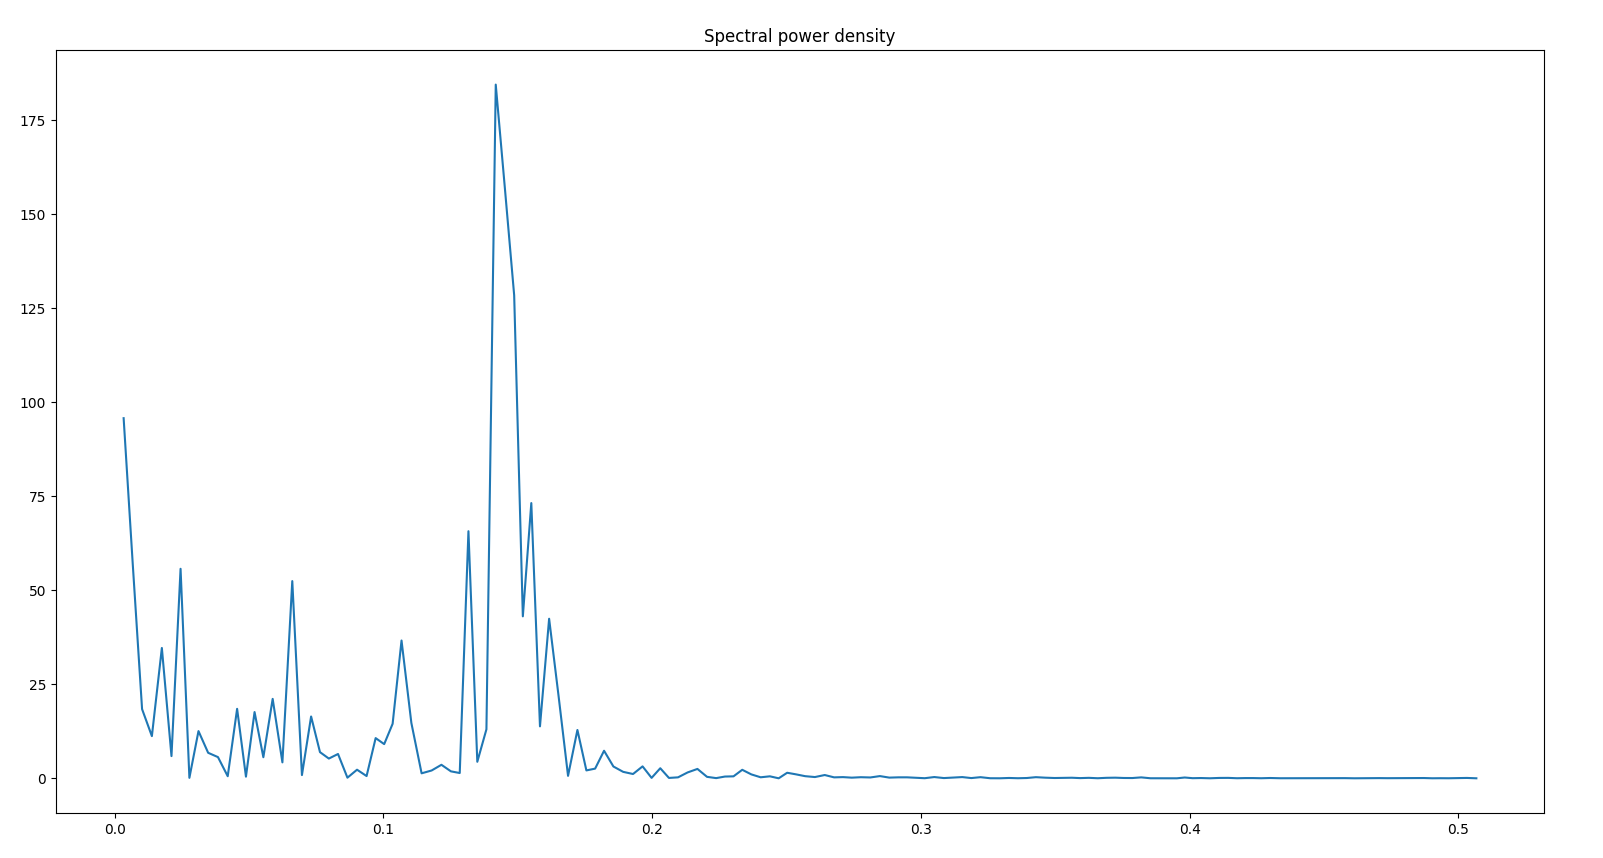
\includegraphics[width=0.8\textwidth]{\jobname/docs/img/spectral-power-density.png}
\end{figure}

\section*{Специфичные диапазоны частот}

Для каждого из специфических диапазонов частот были высчитаны мощности в абсолютной и относительной шкалах.

\subsection*{Высокочастотный диапазон, 0.4 - 0.15, HF}

\begin{align*}
    HF & = 252.382 \\
    HF\% & = 21\%
\end{align*}

\subsection*{Низкочастотный диапазон, 0.15 - 0.04, LF}

\begin{align*}
    LF & = 807.748 \\
    LF\% & = 68\%
\end{align*}

\subsection*{Очень низкочастотный диапазон, 0.04 - 0.015, VLF}

\begin{align*}
    VLF & = 121.381 \\
    VLF\% & = 10\%
\end{align*}

\section*{Суммарная мощность спектра}

Кроме прочего, была высчитана суммарная мощность спектра.

\begin{align*}
    TP & = 1181.511
\end{align*}

\section*{Индексы}

По полученным данным был также рассчитан индекс централизации $IC$, индекс вагосимпатического взаимодействия $IVV$ и
индекс активации подкорковых нервных центров $ISCA$.

\begin{align*}
    IC &= 3.681 \\
    IVV &= 3.2 \\
    ISCA &= 6.655
\end{align*}

\clearpage

\section*{Выводы}

%В ходе выполнения лабораторной работы был исследован набор входных данных с использованием двух подходов:
%автокорреляционный анализа и скаттерографии.
%
%В рамках автокорелляционного анализа была исследована автокорелляционная функция, найдены значения
%$CC0$ и $CC1$ равные соответственно 0.75 и 0.741, а также был построен график автокорелляционной функции.
%
%В рамках скаттерографии (корреляционной ритмографии) была построена скаттерограмма.
%
%Полученный график скаттерограммы представляет собой нормальную форму, которая выглядит, как эллипс, вытянутый вдоль
%биссектрисы.
%Полученное расположение эллипса означает, что к дыхательной прибавлена некоторая величина недыхательной аритмии.
%Помимо прочего, учитывая значение числа сдвигов до первого нулевого значения коэффициента корреляции, можно выдвинуть
%предположение, что в исследуемой выборке доминируют быстроволновые компоненты.

\clearpage

\section*{Листинги}

\subsection*{Листинг основного скрипта}
\lstinputlisting[language=Python,texcl=true]{\jobname/lab3.py}

\subsection*{Листинг утилитного скрипта}
\lstinputlisting[language=Python,texcl=true]{common/common.py}
